\subsection{Conceptual Genesis: Desire and Unsettling}

\emph{Buffalo Soldier} emerges from my father's (and my Uncle's, his brother, to some degree) fascination with the history and depictions of Buffalo Soldiers and Black Cowboys. And I suppose, now  by extension it is my own obsession and fascination. These are figures who occupied complex positions within American imperial expansion, simultaneously agents of and subjected to systems of violent domination. Growing up, I absorbed his interest in these historical figures via the many paintings and memorabilia (a Colt model 1860 six-shooter revolver replica and officer/cavalry sword replicas) adorning many spaces of our home. But it was only through my own research that I began to understand the deeper pattern: the co-commodification of Black bodies and nature by government and military-industrial complexes from the inception of the Buffalo Soldier regiments in the 1860s through to the present (although Buffalo soldiers were disbanded following the Korean War desegregation of the US Army, black soldiers still exist). The term "Buffalo Soldier" itself carries this doubled history, a name given by Indigenous peoples, referencing either the soldiers' fierce fighting or the texture of their hair resembling buffalo fur, depending on which historical account one follows. Either way, the name binds Black bodies to the American buffalo (bison) through colonial violence.

The speculative narrative at the heart of this work imagines an encounter: a Buffalo Soldier meets an American buffalo, and in that meeting, they recognize each other. They share a memory of harvest, slaughter, and rebirth. Both of them commodified, both nearly driven to extinction, both carrying the weight of genocidal logics enacted upon their bodies. This narrative refuses the historical positioning of Buffalo Soldiers as simple heroes or villains, instead locating them within the larger machinery of extraction and elimination that treated both Black bodies and the natural world as resources to be exploited. The work asks: what sonic form can carry this shared memory? How can tactility and material substrate communicate historical fact and speculation simultaneously?

\subsection{Material and Sonic Form: Signal and Remixing}

\begin{figure}[H]
	\centering
	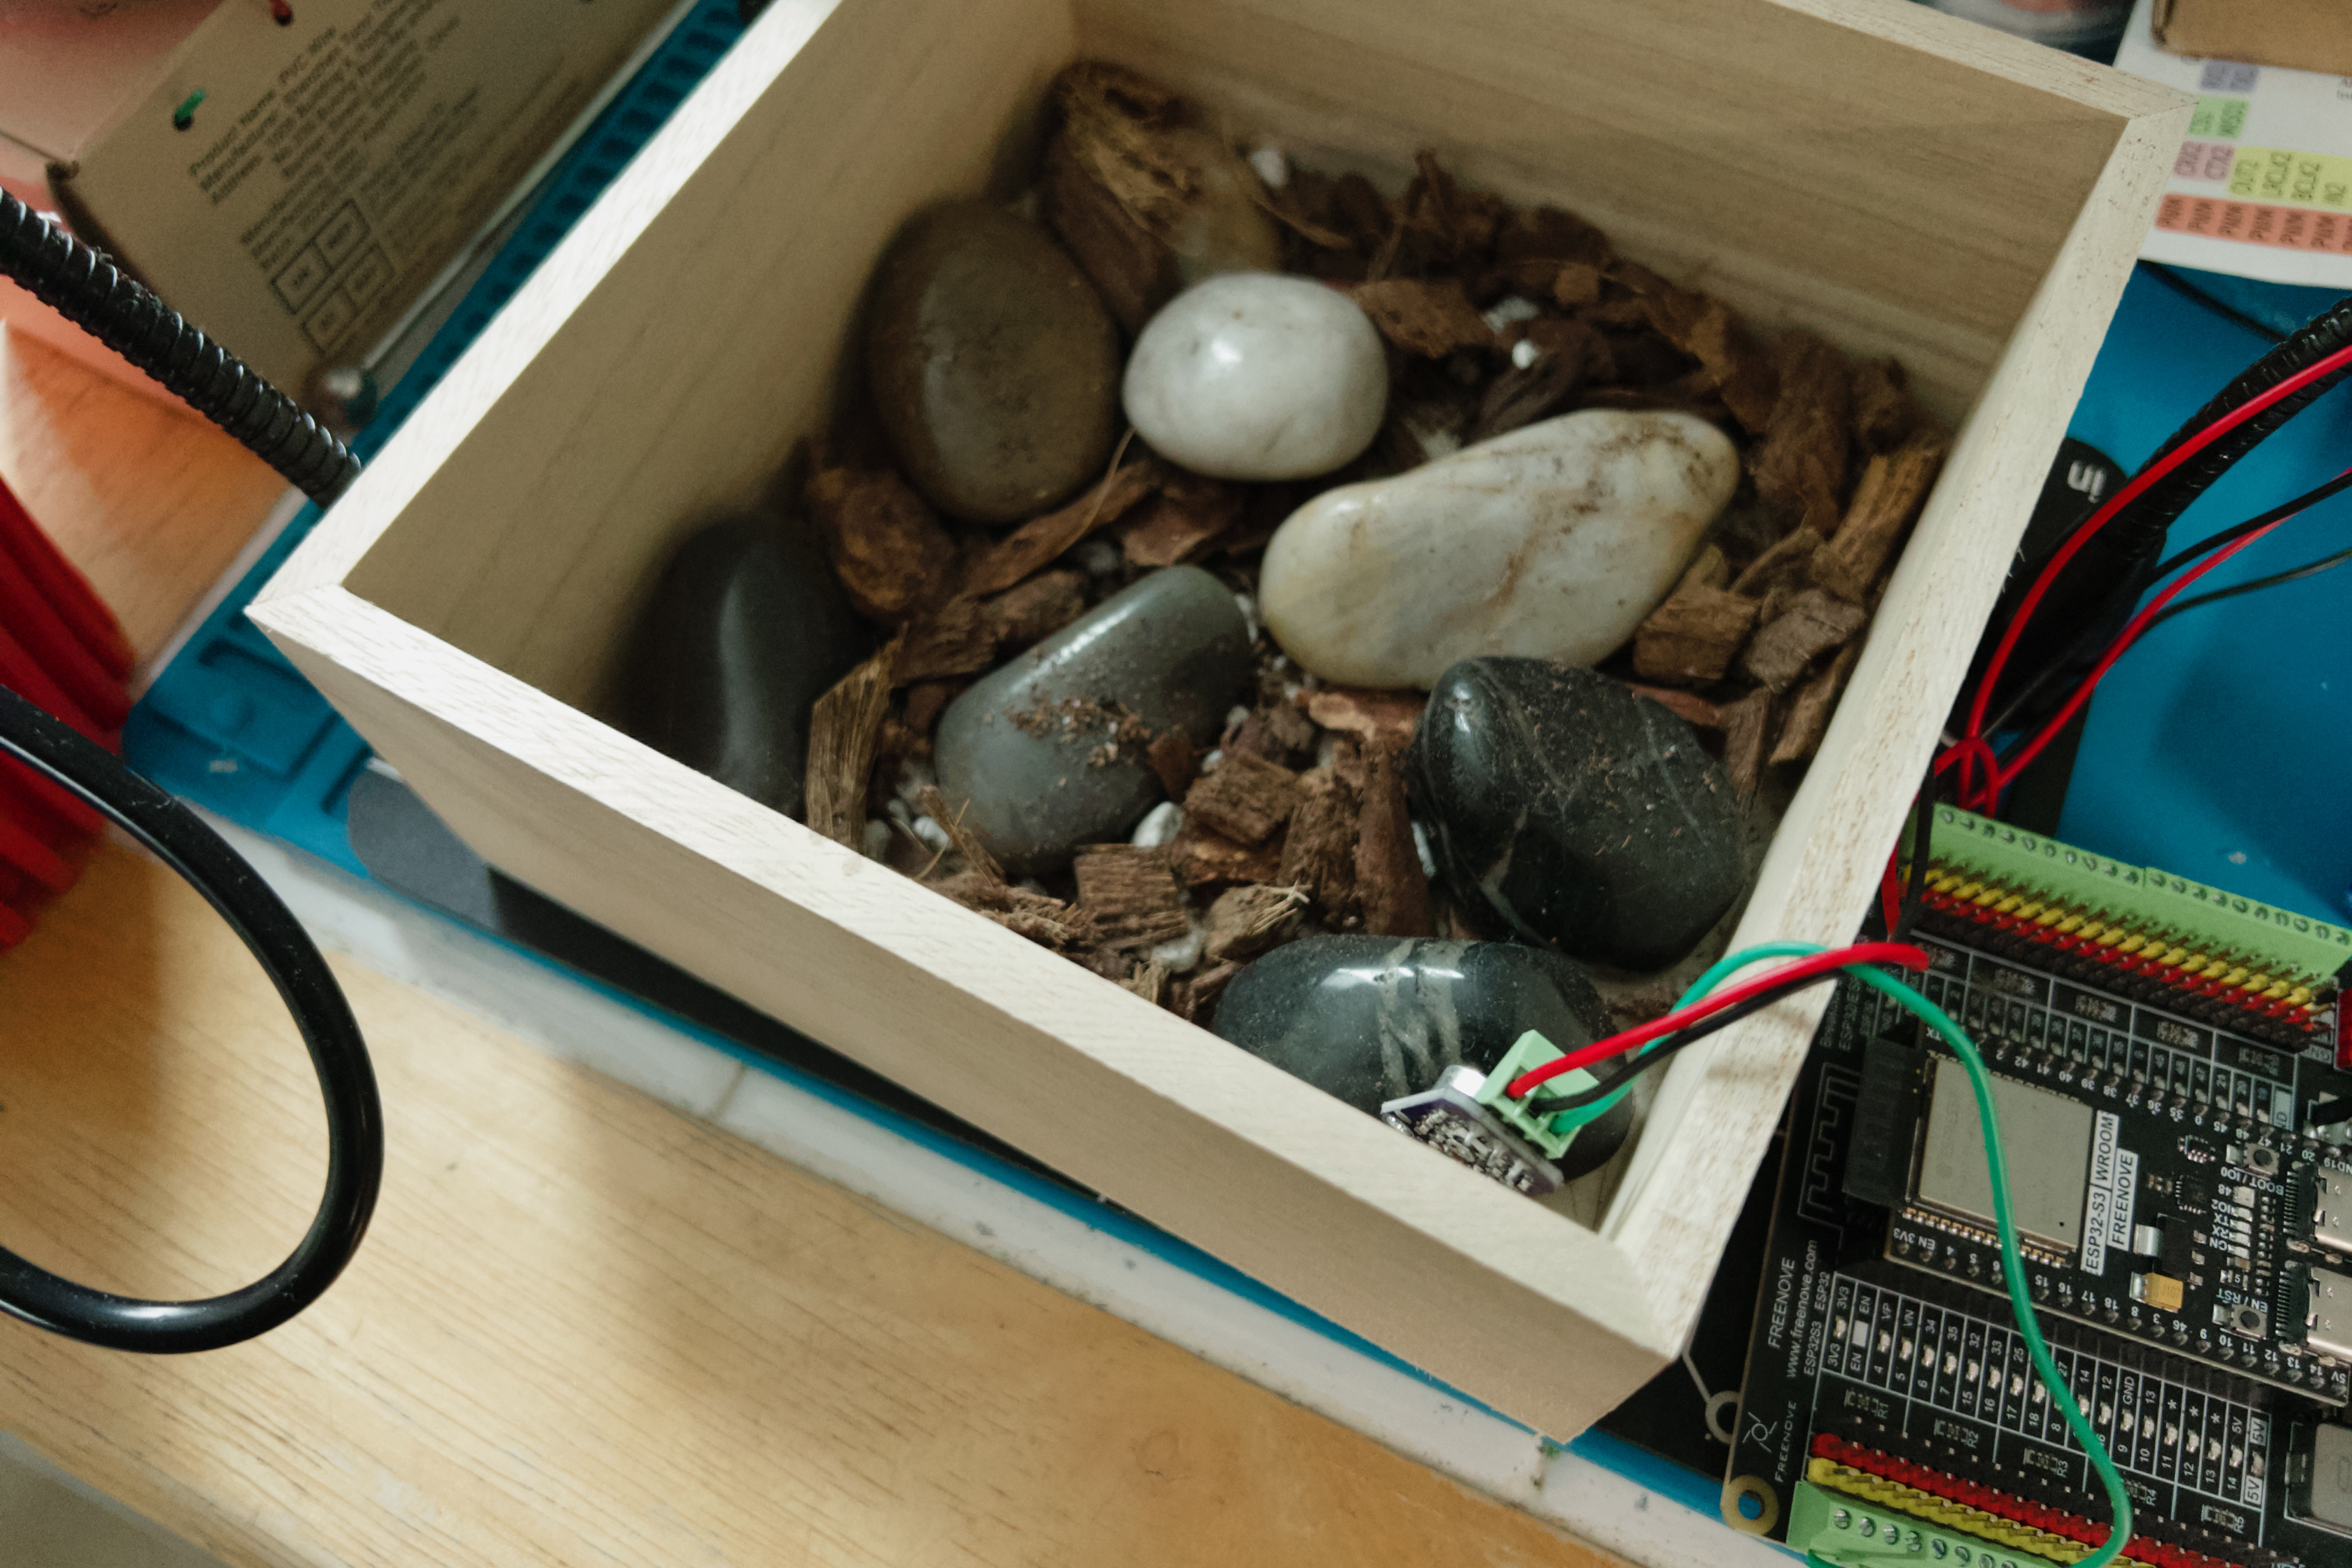
\includegraphics[width=0.7\textwidth]{assets/figures/buffalo_substrate_box.jpg}
	\caption{Wooden substrate box containing rocks, soil, embedded piezoelectric sensor and electret microphone.}
	\label{fig:buffalo-box}
\end{figure}

The primary physical component of \emph{Buffalo Soldier} are wooden boxes containing rocks, soil, and other earth materials embedded with piezoelectric sensors and contact microphones. This is actually a further extension from and earlier iteration to weave a "sonic tapestry" of material substrate. The ritualistic intention for this work is participants interact by touching, striking, or otherwise manipulating the substrate materials. This tactile engagement generates vibrations that the sensors capture and translate into sonic material. This is also a kin to the substrate boxes found on foley stages and the "Case Study of the PebbleBox" from \textit{Sonic Interaction Design} \parencite[~203-212]{Franinovic_Serafin_2013}. The choice of substrate is deliberate: for instance, in this first box earth, rock, and soil reference the land itself, the ground traversed by both buffalo herds and military regiments, the burial sites of bodies both human and animal. The wooden box serves dual symbolic function. It is both the earth that holds memory and the container (coffin, cargo hold, reservation boundary) that confines bodies.


In this early version, sensor data routes through a modified Max/MSP patch where I have configured some standard filtering objects for the incoming signals. At this stage there are still many unaccounted for fictions with the work. For starters, it is still using fairly common and conventional reverb and filtering algorithms that simulate more "neutral" acoustic spaces. These are the defaults provided by Max. However, I plan to continue to research and explore, and possibly develop a much more granular processing chain that fragments and layers the substrate vibrations (possibly with some machine learning) in ways that will allow me to much more easily reference historical rupture and sedimentation. Think of it as the sounds being torn apart and slowly reconstituted, mimicking the violence of extraction and the slow work of memory. The hope is also that the spatialization does not follow typical concert-hall or studio models; instead, sounds move through a more open/outdoor space in patterns informed by data extracted from migration routes and forced marches. Treating the rhythmic temporality of the sounds as the circular or fleeing movements of animals and marching soldiers.

\begin{comment}
\begin{figure}[H]
	\centering
	%\includegraphics[width=0.85\textwidth]{assets/figures/buffalo_max_patch.png}
	\caption{Section of the Max/MSP patch showing modified granular processing chain. The grain size and density parameters are mapped to substrate vibration intensity, creating sonic textures that fragment and coalesce in response to tactile interaction. This modification emerged through iterative listening sessions where I adjusted parameters until the sound carried the historical weight the work demands.}
	\label{fig:buffalo-patch}
\end{figure}
\end{comment}

\subsection{Embodied Development: What Has Emerged}

The development of \emph{Buffalo Soldier} has been iterative and often surprising at times. Early experiments with the substrate box revealed that different materials produce radically different sonic characters (dependent of how they were manipulated within the box). Smooth river rocks create sharp, percussive attacks, while soil and sand generate dense, noisy textures. I have explored how one could manipulate the materials via another mediated layer, like a custom make "piezo wand." But for now simply using the hands feels best for the work. I did find myself drawn to combinations that produce some sonic ambiguity, where it becomes difficult to distinguish whether you are hearing stone striking stone or something more organic. This ambiguity feels essential to the work's intention: the blurring of boundaries between human and animal, between earth and body. Other boxes will likely follow suit and present a "mix" of materials fo the desired sonic qualities to emerge.

As may be obvious, the work remains in active development. Current challenges include refining the sensitivity thresholds for the piezoelectric sensors (too sensitive and ambient vibrations trigger unwanted sounds; not sensitive enough and subtle interactions go unregistered) and expanding the spatial audio system to support more complex multi-channel configurations, more substrate boxes, and the triggering of audiovisual elements in sequences. I am also experimenting with incorporating field recordings, sounds of wind, distant thunder, or even trying to some foley to create "hoof beats." Ultimately, these will likely be layered beneath the substrate-generated material. The direction this takes will depend on what the practice reveals through continued iteration and reflection on historic data and signals.

\subsection{ST Domain Integration}

\textbf{Fugitive Speculation (FS):} \emph{Buffalo Soldier} refuses the dominant narrative that positions Buffalo Soldiers solely as either heroic figures or complicit agents of genocide. Instead, it speculatively imagines a moment of recognition between soldier and buffalo. A form refusal of the separation/segregation that colonial logic often demands. The work speculates on shared memory as a form of resistance to historical erasure.

\textbf{Material Memory (MM):} The substrate materials are intended to carry sedimented memory. The choice to use tactile interaction as the primary input modality grounds the work in embodied gesture, requiring participants to physically touch the materials that reference burial, migration, and confinement.

\textbf{Sensory Worlding (SW):} The work demands multisensory engagement: participants must touch to generate sound, must move through space to experience the spatialization, must attend to both the materiality of the substrate and the sonic transformations their interactions produce. The modified spatialization intended to create a sensory environment informed by movement patterns of migration and data.

\textbf{Intimate Witnessing (IW):} The work's effectiveness depends on whether participants can sense the historical weight encoded in the sonic transformations. Whether the granular fragmentation "feels like" rupture, shrinkage,a nd degradation. Whether the spatial movements evoke the experience of forced migration. This cannot be validated through technical metrics alone (not in the holistic sense of experience); it requires vulnerable sharing with witnesses who can recognize cultural resonance or its absence.